\chapter{Business Model}

\begin{center}
    \textit{Cos'\`e un Business Model?}
\end{center}

\noindent Descrive come un'azienda crea, consegna e cattura valore.\
Ma come si fa a dire queste cose di un'azienda?\ Attraverso i \textbf{Business Model Canvas}, possiamo utilizzarli in molti modi, possiamo prendere un canvas:\ vuoto e un'azienda esistente e provare e riempirlo oppure costruirne uno per una startup.

\begin{figure}[H]
    \centering
    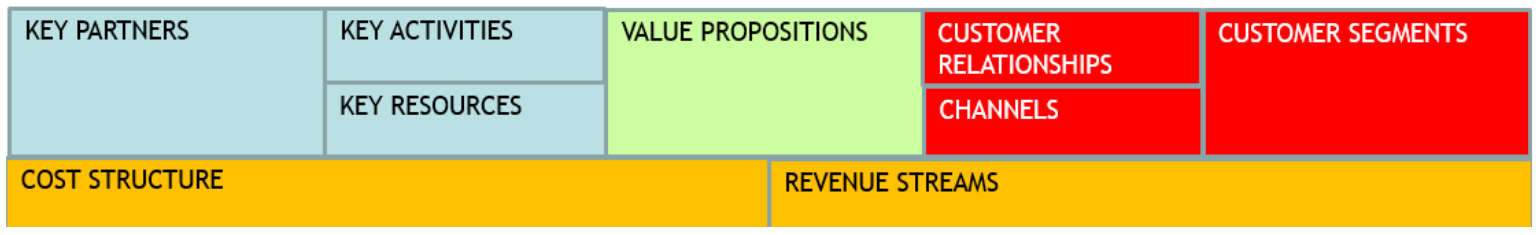
\includegraphics[width=\textwidth]{immagini/BusinessModelCanvas.png}
\end{figure}

\begin{itemize}
    \item \textbf{Customer Segment}:\ Il target di mercato, quali tipi di clienti vogliamo attirare.
    \item \textbf{Value Proposition}:\ Qual è il valore del nostro servizio?\ Cosa offriamo al cliente?\ Per cosa dovrebbero venire da noi?
    \item \textbf{Channels}:\ I canali con cui il servizio arriva ai clienti (shop online, negozio fisico\dots)
    \item \textbf{Customer Relationship}:\ Sembra opzionale ma in realtà il rapporto col cliente è molto importante, ci sono aziende che si focalizzano molto su questo aspetto sfruttando la “fidelizzazione” attraverso dei punti per il cliente.
    \item \textbf{Revenue Streams}:\ I flussi da cui arrivano le entrate, ne descrive anche il tipo.
    \item \textbf{Key Resources}:\ Risorse chiave, le risorse che eroghiamo e che sono fondamentali.
    \item \textbf{Key Activites}:\ L'attività principale della nostra azienda.
    \item \textbf{Key Partnership}:\ È bene cercare dei partner, come Dropbox aveva Amazon, però se il partner fallisce rischia di cadere tutto.
    \item \textbf{Cost structures}:\ Indica quali sono le uscite.
\end{itemize}

\subsubsection{Esempio di Business Model:\ Nespresso}

\begin{figure}[H]
    \centering
    \includegraphics[width=\textwidth]{immagini/NestléBM.png}
\end{figure}

\noindent Nel 1976 Nestl\'e dominava il market con Nescafè il caffè solubile più venduto.\
Le macchinette Nespresso furono ideate nel 1976 quando nessun altro le faceva, erano pronte ma non riuscivano ad entrare nel mercato.\

Nel 1988 il nuovo CEO cambiò il business model, cambiò il \textbf{Customer Segment} poiché le macchinette non dovevano avere lo stesso mercato del Nescaf\'e ma dovevano attrarre impiegati di alto livello e in generale famiglie benestanti.\

\begin{itemize}
    \item Pubblicità:\ l'idea è che sei fig* se bevi Nescaf\'e (vedi George Clooney).
    \item Canali di acquisto:\ online shop, Club Nespresso, oppure vai nelle boutique solo di capsule della Nespresso, solitamente nel centro della città vicino a Armani, Gucci,\ \dots
    \item Club Nespresso:\ una delle cose più importanti per un'azienda è conoscere il comportamento dei propri clienti per riuscire a mantenerli.\ Analisi dei dati, Nespresso traccia il 100\% delle attività dei clienti poich\'e ci sono solo due canali.\ Ogni volta che fai l'ordine col club nespresso vedono tutto quello che hai comprato in modo da poterti offrire tramite newsletter e news i prodotti più adatti.
\end{itemize}

\noindent Dal punto di vista della sostenibilità ambientale Nespresso produce una grandissima quantità di materiale difficilmente riciclabile che attualmente viene smaltito male.\
Come la commercializzazione del latte in polvere, grande successo di Nestl\'e, ma ha avuto effetti secondari:\ nei paesi in via di sviluppo l'acqua con cui veniva sciolto il latte era contaminata e molti bambini sono morti.\
Hanno conquistato comunque una fetta di mercato importante.

\subsubsection{Esempio di Business Model:\ Zara}

Zara ha deciso di produrre abiti in base a cosa la gente acquista, non è il cliente a seguire la moda ma è Zara a seguire il cliente.\ Rinnova continuamente.\
\textbf{No warehousing:\ no magazzino, viene spedito quello che serve ad ogni negozio}.\

\subsubsection{Esempio di Business Model:\ TicketResturant}

\textbf{Idea}\quad Le piccole imprese acquistano buoni e li distribuiscono ai dipendenti; i dipendenti riscattano i voucher presso i ristoranti locali
\vspace{12pt}

\noindent Guadagna da entrambe le parte:\
il datore di lavoro paga un premio sull'importo del buono, mentre il commerciante incassa con uno sconto sull'importo del buono.\
Rottura (buoni emessi ma non utilizzati).\
Reddito fluttuante (intervallo tra l'acquisto del voucher e il rimborso del voucher).\

\section{Freemium come Business Model}

Consiste in una suddivisione dei servizi:\ una parte \textbf{Free} che comprende cosiddetti i servizi ``di base'' e una parte \textbf{Premium} a pagamento che invece offre servizi aggiuntivi e/o migliorati.\
Chi adotta il modello Freemium deve porre molta attenzione al costo che comportano gli utenti ``free'' e alla percentuale di conversione degli utenti che decidono di passare a Premium.\
I prossimi esempi metteranno in luce quali sono i modi in cui guadagnano le aziende che seguono questo modello.

\subsubsection{Flickr}

\begin{figure}[H]
    \centering
    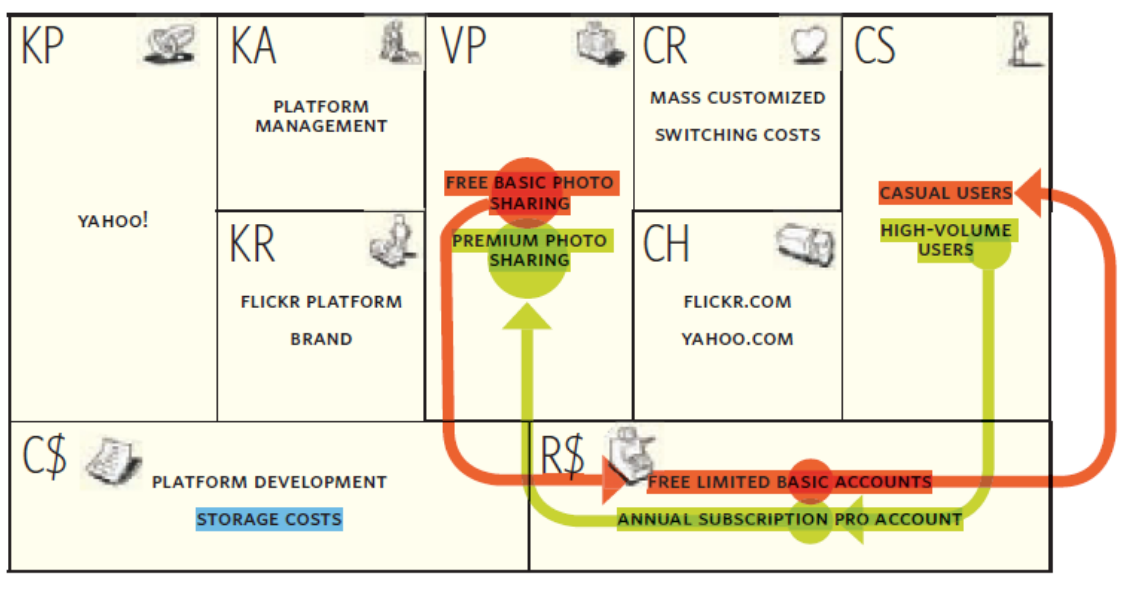
\includegraphics[width=0.7\textwidth]{immagini/Flickr.png}
\end{figure}

Se paghi puoi avere premium photo sharing:\ oltre a poter organizzare foto in cartelle, si ottengono dei servizi addizionali.\

È durato 3 anni, dal 2002 al 2005, acquistato da Yahoo per 25 milioni di dollari che a sua volta è stato acquistato da Verizon per 4 miliardi nel 2017 dopo aver rifiutato 44 miliardi da Microsoft nel 2009.\

\subsubsection{RedHat}

\begin{figure}[H]
    \centering
    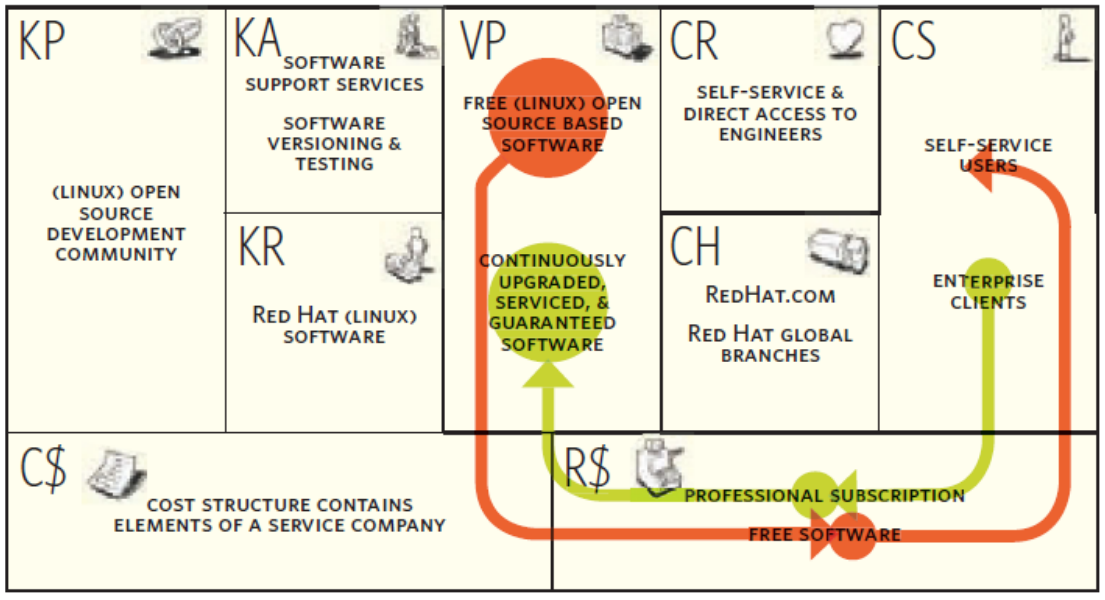
\includegraphics[width=0.7\textwidth]{immagini/RedHat.png}
\end{figure}
Chi usava un open source e offriva un servizio aveva paura che l'open source fallisse, RedHat si metteva nel mezzo e garantiva stabilità, veniva pagato e manteneva l'open source sempre aggiornato:\ open source non significa che il software sia gratuito ma che è possibile modificarne il sorgente.\

Venduto per 34 miliardi di dollari a IBM.\

\subsubsection{Skype}

\begin{figure}[H]
    \centering
    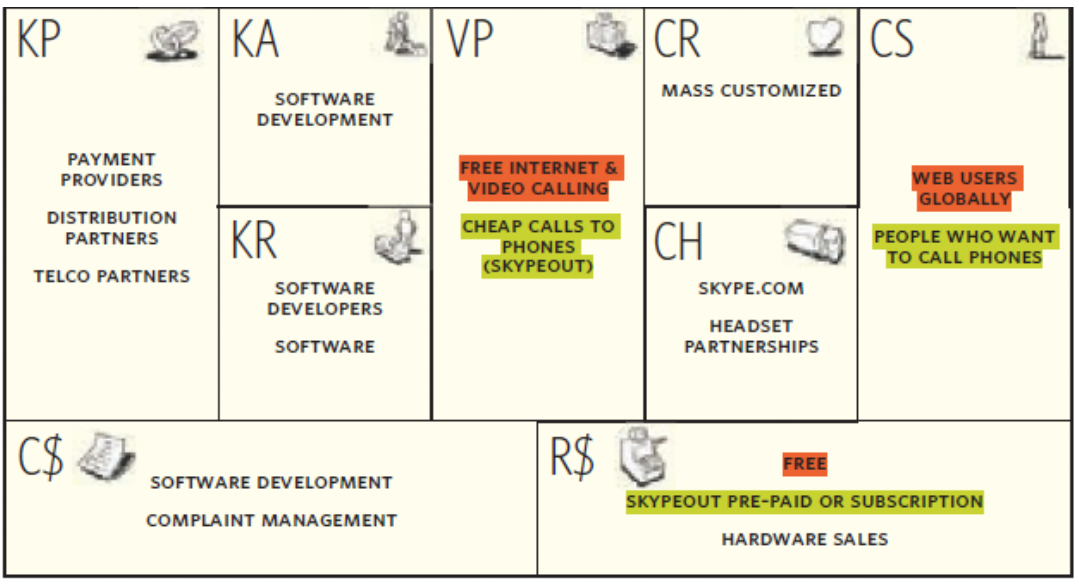
\includegraphics[width=0.7\textwidth]{immagini/Skype.png}
\end{figure}

Tutti gli utenti web possono fare chiamate gratuite e anche videochiamate.\
Pagando si ha la possibilità di chiamare anche i cellulari a prezzi competitivi.\

Nato nel 2003, comprato da Ebay nel 2005 e poi nel 2011 da Microsoft.

\subsubsection{Dropbox}

Dropbox ha 500 milioni di utenti di cui 12 milioni paganti.

\begin{table}[H]
    \centering
    \begin{tabular}{|l|l|}
        \hline
        \multicolumn{2}{|c|}{\textbf{Privati}}      \\\hline\hline
        Free:         & 2 GB                        \\
        Plus:         & 1 TB per €9,99 al mese      \\
        Professional: & 2 TB per €19,99 al mese     \\
        \hline\hline
        \multicolumn{2}{|c|}{\textbf{Aziende}}      \\\hline\hline
        Standard:     & 3TB per €10,00 al mese      \\
        Adavanced:    & no limit per €15,00 al mese \\
        Enterprise:   & ``contact us''              \\\hline
    \end{tabular}
\end{table}

\subsubsection{Neflix}

Netflix usa attualmente il \textbf{15\% del traffico internet} in download nel mondo.\
Paga i diritti dei film e guadagna per il ``noleggio'' verso gli utenti.\
Come già detto, Dropbox ha iniziato appoggiandosi ad Amazon AWS e poi si è distaccato; Netflix invece ha iniziato la partnership con Amazon, nonostante avesse costruito già i data center.\
L'arrivo dei Container ha creato dei problemi al reparto di sviluppo di Netflix e alla fine hanno dovuto mettere da parte l'idea di usare i propri data center chiudendoli e continuando ad appoggiarsi ad Amazon.\

\section{Business Model Generation}

Esistono diversi tipi di strategie per i Business Model.\
Al giorno d'oggi la cosa più importante è mettere al centro il cliente e il rapporto che si crea con esso:\ bisogna chiedersi di che cosa ha bisogno, come preferisce essere contattato, a quale tipo di valore sono interessati i clienti e per cosa sono diposti a pagare.\
Per innovare il business model si può\dots
\begin{itemize}
    \item Partire dalle risorse che ha già l'azienda (\textbf{Resource Driven}), come ad esempio \textbf{Amazon Fulfillment} che consiste nell'offrire a terze parti la possibilità di vendere e far arrivare i propri beni ai clienti.\ Prima di iniziare con questa pratica Amazon aveva già tutto pronto (shop online, catena organizzativa).
    \item Basarsi sull'offerta (\textbf{Offer Driven}), ad esempio:\ \textbf{Cemex} che in un momento in cui il cemento era garantito in 48h di tempo è riuscita a farlo in 4h.
    \item Basarsi sui clienti (Customer Driven):\ \textbf{23andMe} offriva test per dna ai singoli clienti privati.
    \item Basarsi sull'aspetto finanziario (\textbf{Finance Driven}), per esempio \textbf{Xerox} che introdusse un modello in cui il costo delle fotocopie veniva offerto in leasing e venivano inoltre garantite 2000 copie gratuite.
    \item Epicentri multipli (Multiple Epicenter Driven):\ sono tutti modi in cui si può ridefinire un Business Model innovativo partendo da angolature distinte.\ Le idee delle aziende che hanno fatto più successo (Google, Spotify, Dropbox,\ \dots) si sono basate su domande del tipo ``Cosa succederebbe se offrissi musica gratis a tutti?''\ e sono riuscite a trovare una strategia vincente.\
\end{itemize}

\subsection{Statistiche startup}
\textbf{Airbnb}:\ valore di 35 miliardi di dollari.\
2 Milioni di persone a notte dormono in una struttura prenotata su Airbnb.\

\noindent \textbf{Epic Games}:\ Fortnite ha 250 Milioni di giocatori e guadagna centinaia di milioni di dollari al mese grazie alla vendita delle skin.

\noindent \textbf{Facebook}:\ 2.45 miliardi di persone ogni mese.

\noindent \textbf{Instagram}:\ acquistato da Facebook dopo 2 anni per un miliardo di dollari.

\vspace{12pt}
\noindent Il 90\% delle startup fallisce per 4 motivi principali:\ incompetenza, incapacità di gestire il budget, mancanza di esperienza, problemi personali.

\subsubsection{Spotify}

Il nome è nato da un misunderstanding.\
Gli stakeholder di spotify sono:

\begin{itemize}
    \item Freeusers
    \item Royalty holder:\ quelli che vengono pagati ogni volta che viene riprodotto un brano (SIAE in Italia).
    \item Subscriber:\ utenti premium.
    \item Advertiser:\ coloro che pagano Spotify per venire sponsorizzati.
\end{itemize}

\noindent Gli utenti free e gli utenti abbonati devono bilanciarsi, ma quando iniziamo con un modello Freemium non abbiamo idea di quale sarà la percentuale tra utenti free e premium, è difficile da stabilire.\

Spotify per pagare meno di royalty ha ideato una strategia che permette di scegliere dove reperire il brano in base alla localizzazione dell'utente poiché i costi variano in base al paese da dove l'utente richiede l'ascolto.\

Se gli utenti Premium ascoltano troppo rischiamo di andare in perdita poiché è più quello che paghiamo per le royalties che quello che riceviamo dagli utenti.\

\begin{table}[H]
    \centering
    \begin{tabular}{|l|}
        \hline
        \multicolumn{1}{|c|}{\textbf{Statistiche:}} \\\hline\hline
        217 milioni di utenti attivi                \\
        100 milioni di questi sono membri Premium   \\\hline
    \end{tabular}
\end{table}

\subsection{Casi di studio}

\subsubsection{Le entrate di Amazon (Amazon revenue)}
Le entrate di Amazon nel 2019  sono state pari a \textbf{280 miliardi di dollari}.\
\begin{enumerate}
    \item Store Online
    \item Venditore per altri (Amazon Fulfillment)
    \item Amazon Web Services (Cloud)
\end{enumerate}

\subsubsection{Le entrate di Google}
Google è un servizio gratuito, come fa a guadagnare?\ Grazie al Customized Advertising, la nostra ``attenzione'' verso le pubblicità permette a Google di farsi pagare.\

\noindent Cinque Riflessioni sui motori di ricerca
\begin{itemize}
    \item Per la prima volta nella storia tutti posiamo facilmente generare informazioni accessibili a tutti.\ Ci sono più di \textbf{4 miliardi di utenti su Internet e quasi 2 miliardi di siti Web}.\ Quasi tutte le ricerche di informazioni passano attraverso un unico punto di accesso:\ Google.\ Azienda che domina il mondo dei motori di ricerca con più di \textbf{3.5 miliardi di ricerche} giornaliere.\
          Durante una ricerca \textbf{i primi 3 risultati ottengono il 75\% dei click} e solitamente se non troviamo niente nei primi 3 risultati cambiamo query di ricerca.\ I siti Web cercano di comparire nei primi 3 risultati perché altrimenti non vengono cliccati.\ Dobbiamo sempre tenere a mente che la prima pagina dei risultati di Google è una parte molto piccola di tutte le informazioni esistenti.\
    \item \textbf{Google non controlla le fonti, né se un'informazione è vera o no}.\ Se facciamo una ricerca oggi nei primi 3 risultati otteniamo determinati siti web, se riprovassimo a cercare la stessa cosa dopo un mese potremmo avere dei risultati diversi.
    \item Google può \textbf{tenere traccia} delle nostre attività poiché possiede molti servizi diversi:\ Youtube, Google Maps, Google Chrome, Google Shopping, Google Calendar, Waze, Google Photos,\ \dots
    \item Cosa succederebbe se Google manipolasse i risultati delle ricerche?\ È stato fatto un esperimento ed è stato osservato che è possibile spostare le preferenze di voto degli elettori indecisi del 20\% mostrando degli opportuni risultati di ricerca (in modo trasparente) agli utenti.
    \item Quali sono gli effetti di Google per la nostra memoria?\ Se sappiamo che possiamo avere accesso a certe informazioni in qualsiasi momento non le ricordiamo, ma ci limitiamo a ricordare dove possiamo cercarle o trovarle.\ Questa cosa si chiama \textit{memoria transattiva} ed è sempre esistita:\  sapere che ci sono cose che non si ricordano, ma sapere che altre persone invece le sanno.\ \textbf{Internet diventa una \textit{memoria transattiva}}.
\end{itemize}

